%=============================================================================
%  FinITR-AI : IEEE conference paper (IEEEtran, two-column)
%  Compile with pdfLaTeX on Overleaf. Figures live in ./images/
%  NOTE for the author: fill the author block placeholders (<< ... >>) before
%  submission. Every numeric result here is taken from the project's stored
%  evaluation files; do not alter a figure without re-checking its source.
%=============================================================================
\documentclass[conference]{IEEEtran}
\IEEEoverridecommandlockouts

\usepackage{cite}
\usepackage{amsmath,amssymb,amsfonts}
\usepackage{graphicx}
\usepackage{textcomp}
\usepackage{xcolor}
\usepackage{booktabs}
\usepackage{array}
\usepackage{url}

\graphicspath{{images/}}

% A neat fixed-width column type for the result tables.
\newcolumntype{C}[1]{>{\centering\arraybackslash}m{#1}}

\begin{document}

\title{FinITR-AI: A Verified Multi-Agent System for Indian Income-Tax Return
Preparation with Deterministic Computation and Notice-Risk Prediction}

\author{
\IEEEauthorblockN{<< Author One >>}
\IEEEauthorblockA{\textit{Dept. of << Department >>} \\
\textit{<< Institute >>}\\
<< City >>, India \\
<< email >>}
\and
\IEEEauthorblockN{<< Author Two >>}
\IEEEauthorblockA{\textit{Dept. of << Department >>} \\
\textit{<< Institute >>}\\
<< City >>, India \\
<< email >>}
\and
\IEEEauthorblockN{<< Supervisor >>}
\IEEEauthorblockA{\textit{Dept. of << Department >>} \\
\textit{<< Institute >>}\\
<< City >>, India \\
<< email >>}
}

\maketitle

\begin{abstract}
Preparing an Indian income-tax return forces a taxpayer to reconcile several bank
accounts against the Annual Information Statement, settle on a tax regime, pick
the right form, and apply slab rules that change almost every year. Commercial
filing tools handle the well-trodden salaried path but cannot explain
themselves or reason about a mismatch, while general large language models answer
fluently yet make confident arithmetic mistakes on the current year's slabs. We
present FinITR-AI, a system that keeps the language model away from the
arithmetic. Four cooperating agents---an Auditor, an Optimizer, a Compliance
checker, and a Critic---reason over a shared context, but every figure is
produced by a deterministic engine pinned to the FY~2025-26 rules, and a Critic
agent verifies each claim against the source documents and a structured tax-law
corpus, blocking any unsupported claim and forcing a bounded re-run. The whole
pipeline runs offline so that no financial document leaves the user's machine.
On IndianTaxBench, a 140-case benchmark we built for the task, FinITR-AI reaches
94.0\% tax-computation accuracy while holding its hallucination rate at 6.8\%,
against 70--74\% accuracy and 24--27\% hallucination for two strong general
models evaluated on the same prompts. An ablation attributes a 39.8-point share
of the tax accuracy to the deterministic engine alone and shows the Critic, not
the model, is what suppresses hallucination. We discuss the system's limits
candidly, including a small evaluation scale and a static rule corpus.
\end{abstract}

\begin{IEEEkeywords}
income-tax automation, multi-agent systems, large language models, retrieval
augmentation, hallucination, deterministic reasoning, India
\end{IEEEkeywords}

%=============================================================================
\section{Introduction}
%=============================================================================
Filing a return in India is rarely a single clean calculation. A salaried filer
who also trades on a broker, holds a few fixed deposits, pays rent, and dabbles
in crypto has to pull figures from statements in several formats, line them up
against what the tax department already knows through the Annual Information
Statement (AIS) and Form~26AS, decide between the old and the new regime, and
then choose among a set of forms whose applicability is itself a small puzzle.
A wrong move at the very first step---misreading a credit, or quietly leaving an
AIS entry off the return---is also the most common trigger for a Section~143(1)
notice, which the tax department's own reporting attributes largely to AIS
mismatches~\cite{ref_cbdt}. The cost of an error, in other words, lands on the
taxpayer, not on the tool.

Two kinds of help exist today, and each falls short in a different way. The
assisted-filing products that most people use are accurate within the path their
designers anticipated, but they treat the AIS as a list to be displayed rather
than a quantity to be reconciled, and they cannot say \emph{why} they reached a
conclusion. General-purpose language models go to the opposite extreme: they will
discuss any scenario, but when a rule has to be turned into a number they slip,
and they do so with the same confident tone they use when they are right. In a
setting where the output is a figure that will be filed, a fluent wrong number is
worse than a blunt refusal.

This paper describes FinITR-AI, a system built on a single guiding decision:
let the language model reason about \emph{what} to compute, but never let it do
the computing. The contributions are threefold. First, a four-agent architecture
in which an Auditor, Optimizer, Compliance checker, and Critic share one evolving
context, with arithmetic delegated entirely to a deterministic engine carrying
the current year's rules. Second, a verification loop in which the Critic does
more than annotate---it can veto an ungrounded claim and send the responsible
agent back for a bounded re-run. Third, a notice-risk model that turns AIS
reconciliation into an explicit, interpretable probability of scrutiny, a signal
no commercial tool surfaces. We evaluate the system on a purpose-built benchmark
and, equally, we are candid about what the evaluation does not yet establish.

%=============================================================================
\section{Related Work}
%=============================================================================
\subsection{Rule-Based and Commercial Filing Tools}
The income-tax department's own portal and offline utilities are the reference
implementation of the rules; they pre-fill some fields and validate the final
return, but they advise nothing and present the AIS raw~\cite{ref_portal}.
ClearTax and Quicko wrap that machinery in a guided experience, import Form~16,
and compare regimes~\cite{ref_cleartax,ref_quicko}. Their reconciliation of the
AIS against self-reported income is shallow, their reasoning is a closed rule
engine, and neither attaches a natural-language rationale or a quantified notice
risk to its output.

\subsection{Academic Prototypes for Indian Tax Automation}
Two recent prototypes share our goal. Auto~ITR assembles a full pipeline from
bank-statement ingestion to a chartered-accountant export, with a hybrid
rule-and-heuristic categorizer, a statistical anomaly detector, and a
break-even regime optimizer~\cite{ref_autoitr}. It is the more complete deployed
product, but it runs as a single deterministic pass with no component that can
question an earlier conclusion, and its chatbot calls a hosted model. A second
system pairs a rule layer with a retrieval-augmented model whose knowledge base
updates itself by scraping government circulars~\cite{ref_selfrag}; its
self-refreshing corpus is a genuine strength, but its evaluation is qualitative,
it relies on a cloud model, and it reads structured Tally exports rather than the
bank statement and Form~16 that an ordinary salaried filer actually has.

\subsection{Agentic, Tool-Augmented, and Verified Reasoning}
The techniques we build on come from the wider effort to make language models
reliable by letting them act. ReAct interleaves reasoning with tool
calls~\cite{ref_react}; retrieval-augmented generation grounds output in an
external corpus~\cite{ref_rag}. The closest contemporary work tackles
hallucination in financial reasoning directly: a neuro-symbolic system pairs a
deterministic fact ledger with an adversarial hallucination
detector~\cite{ref_venra}, a fine-grained scheme verifies financial answers at
the level of atomic knowledge units~\cite{ref_finrag}, and tool-receipt methods
check whether an agent truly invoked a tool rather than fabricating its
result~\cite{ref_receipts}. An agentic framework has also been applied to
generating and metamorphically testing U.S. tax-prep \emph{software}, a related
but distinct problem~\cite{ref_synedrion}. Our verification loop is a
domain-specific instance of these ideas; what is new here is not the idea of
checking a claim but the assembly---a vetoing critic wired over a deterministic
Indian tax engine, with an interpretable notice-risk model and offline
execution, aimed at end-to-end filing rather than software synthesis or general
financial Q\&A.

%=============================================================================
\section{System Architecture}
%=============================================================================
FinITR-AI is organized as a reasoning loop over a shared \texttt{AgentContext}
object, illustrated in Fig.~\ref{fig:arch}. Documents enter through a set of
parsers; the orchestrator then runs four agents in sequence, each writing its
findings back into the shared context so the next agent sees an enriched picture
rather than the raw input.

\begin{figure}[t]
  \centering
  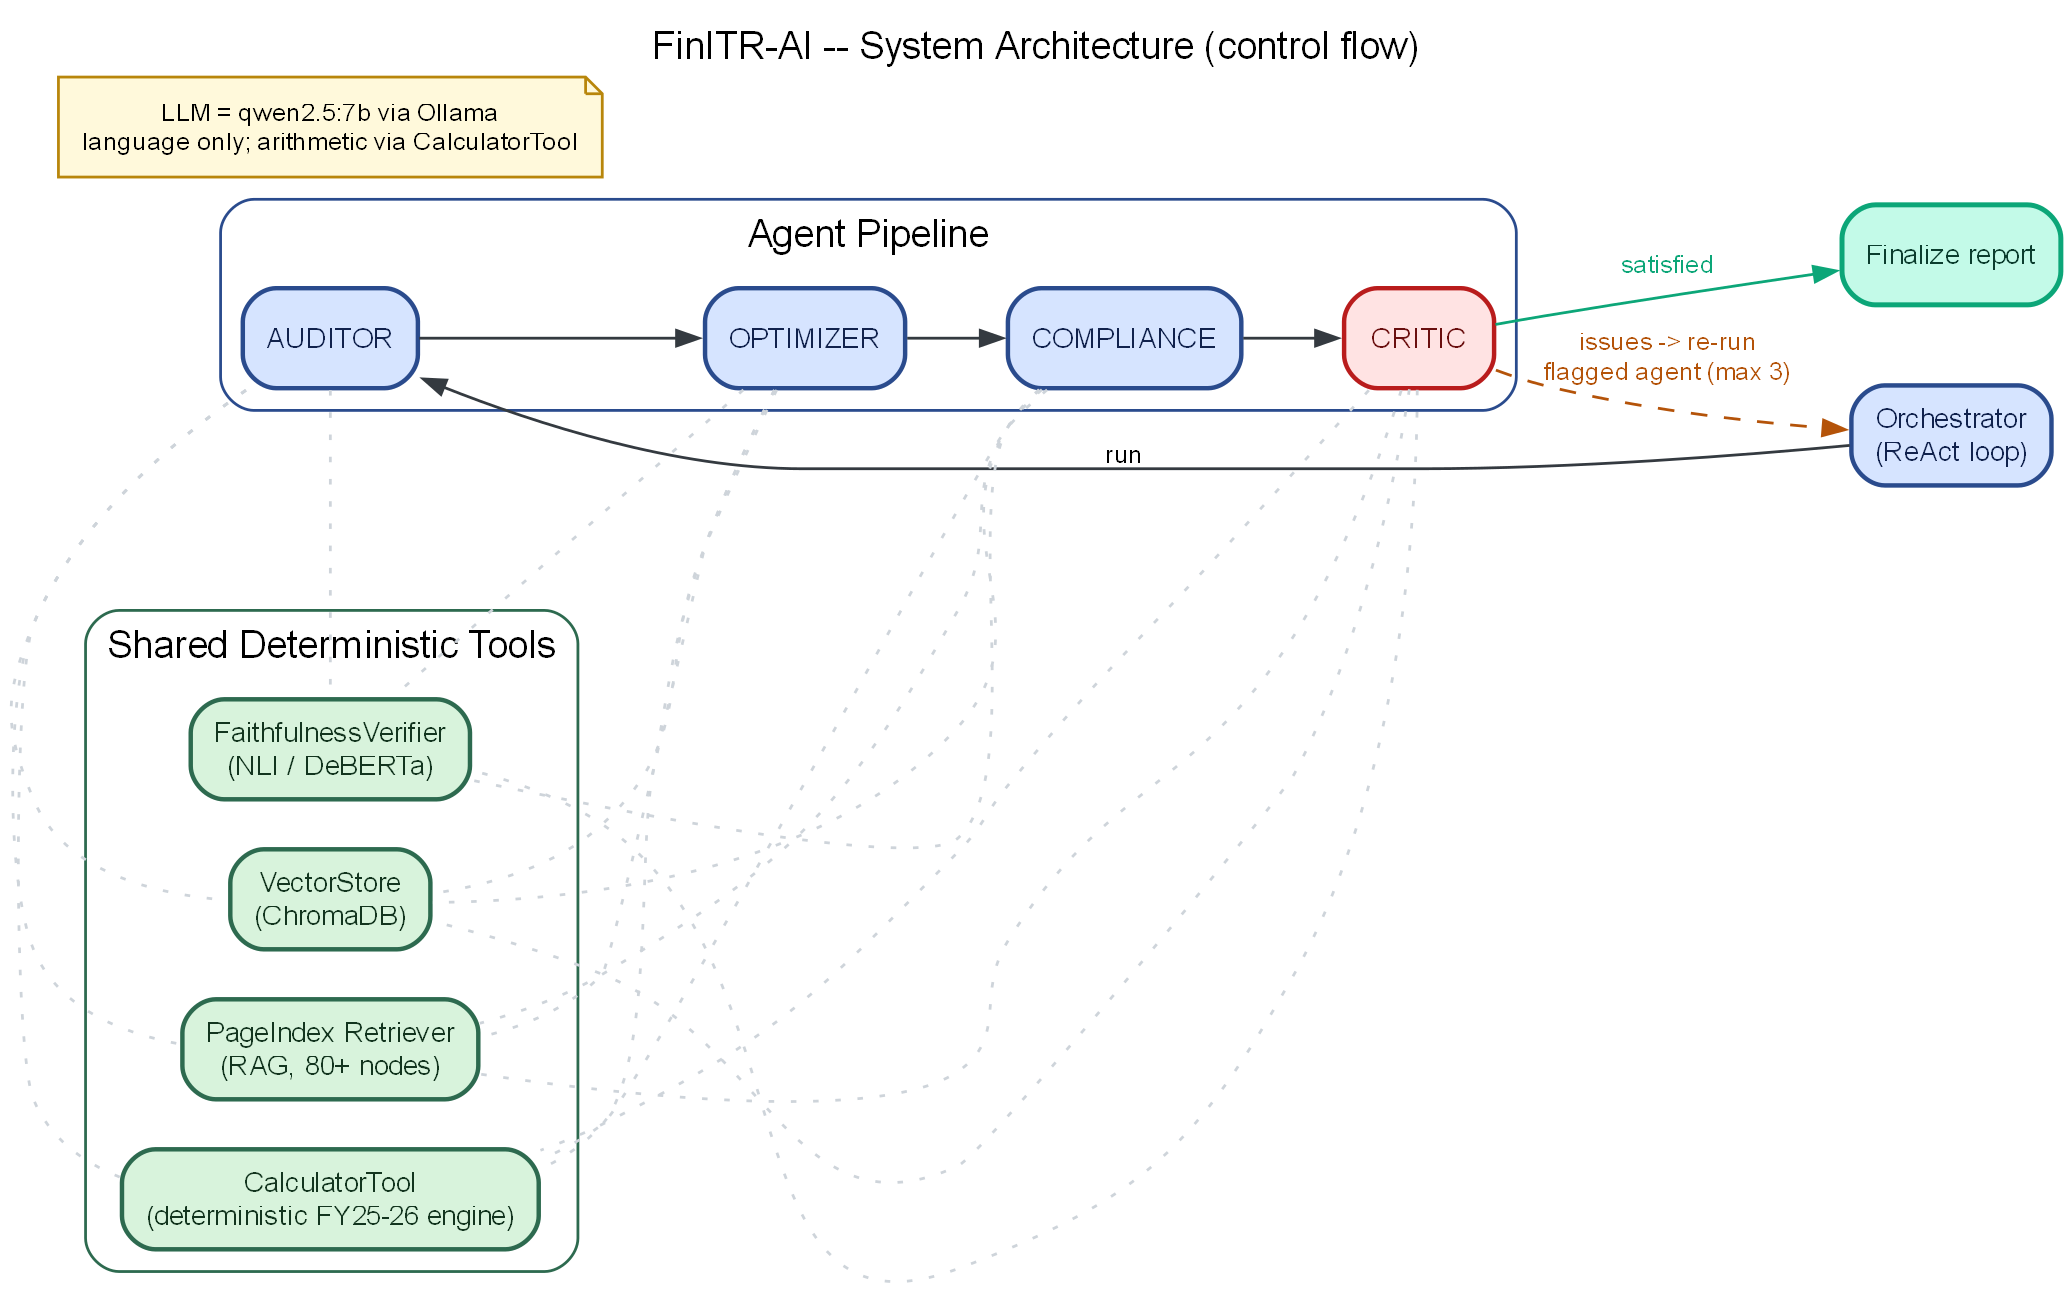
\includegraphics[width=\columnwidth]{architecture.png}
  \caption{FinITR-AI architecture. Four agents reason over a shared context;
  arithmetic is delegated to a deterministic CalculatorTool, and the Critic
  verifies claims against parsed documents and a structured tax-law corpus
  before the return is finalized.}
  \label{fig:arch}
\end{figure}

The \textbf{Auditor} ingests and reconciles. It parses Form~16, Form~26AS, the
AIS, and bank or broker statements, classifies every transaction, and builds an
explicit ledger of items that match across sources, items present only in the
AIS, and items that disagree. The \textbf{Optimizer} computes the liability under
both regimes and recommends the cheaper one, together with deduction headroom the
filer has not yet used. The \textbf{Compliance} agent selects the ITR form and
the schedules the case requires. The \textbf{Critic} is the agent that makes the
output trustworthy: it checks each material claim against the parsed evidence and
a retrieved section of the Income-Tax Act, using a natural-language-inference
cross-encoder~\cite{ref_deberta} to test whether the claim is entailed by its
evidence; when a claim is unsupported it
does not merely flag it---it blocks the claim and triggers a bounded re-run of
the agent responsible, up to a fixed iteration cap so the loop always terminates.

Two design rules hold throughout. No agent ever performs arithmetic; every
number flows through a deterministic CalculatorTool that encodes the FY~2025-26
slabs, rebate, surcharge, cess, and marginal-relief threshold. And nothing leaves
the device: the reasoning runs against a locally hosted model, on the view that
for tax data privacy is closer to a requirement than a feature. Fig.~\ref{fig:flow}
shows the end-to-end data path from upload to the assembled return.

\begin{figure}[t]
  \centering
  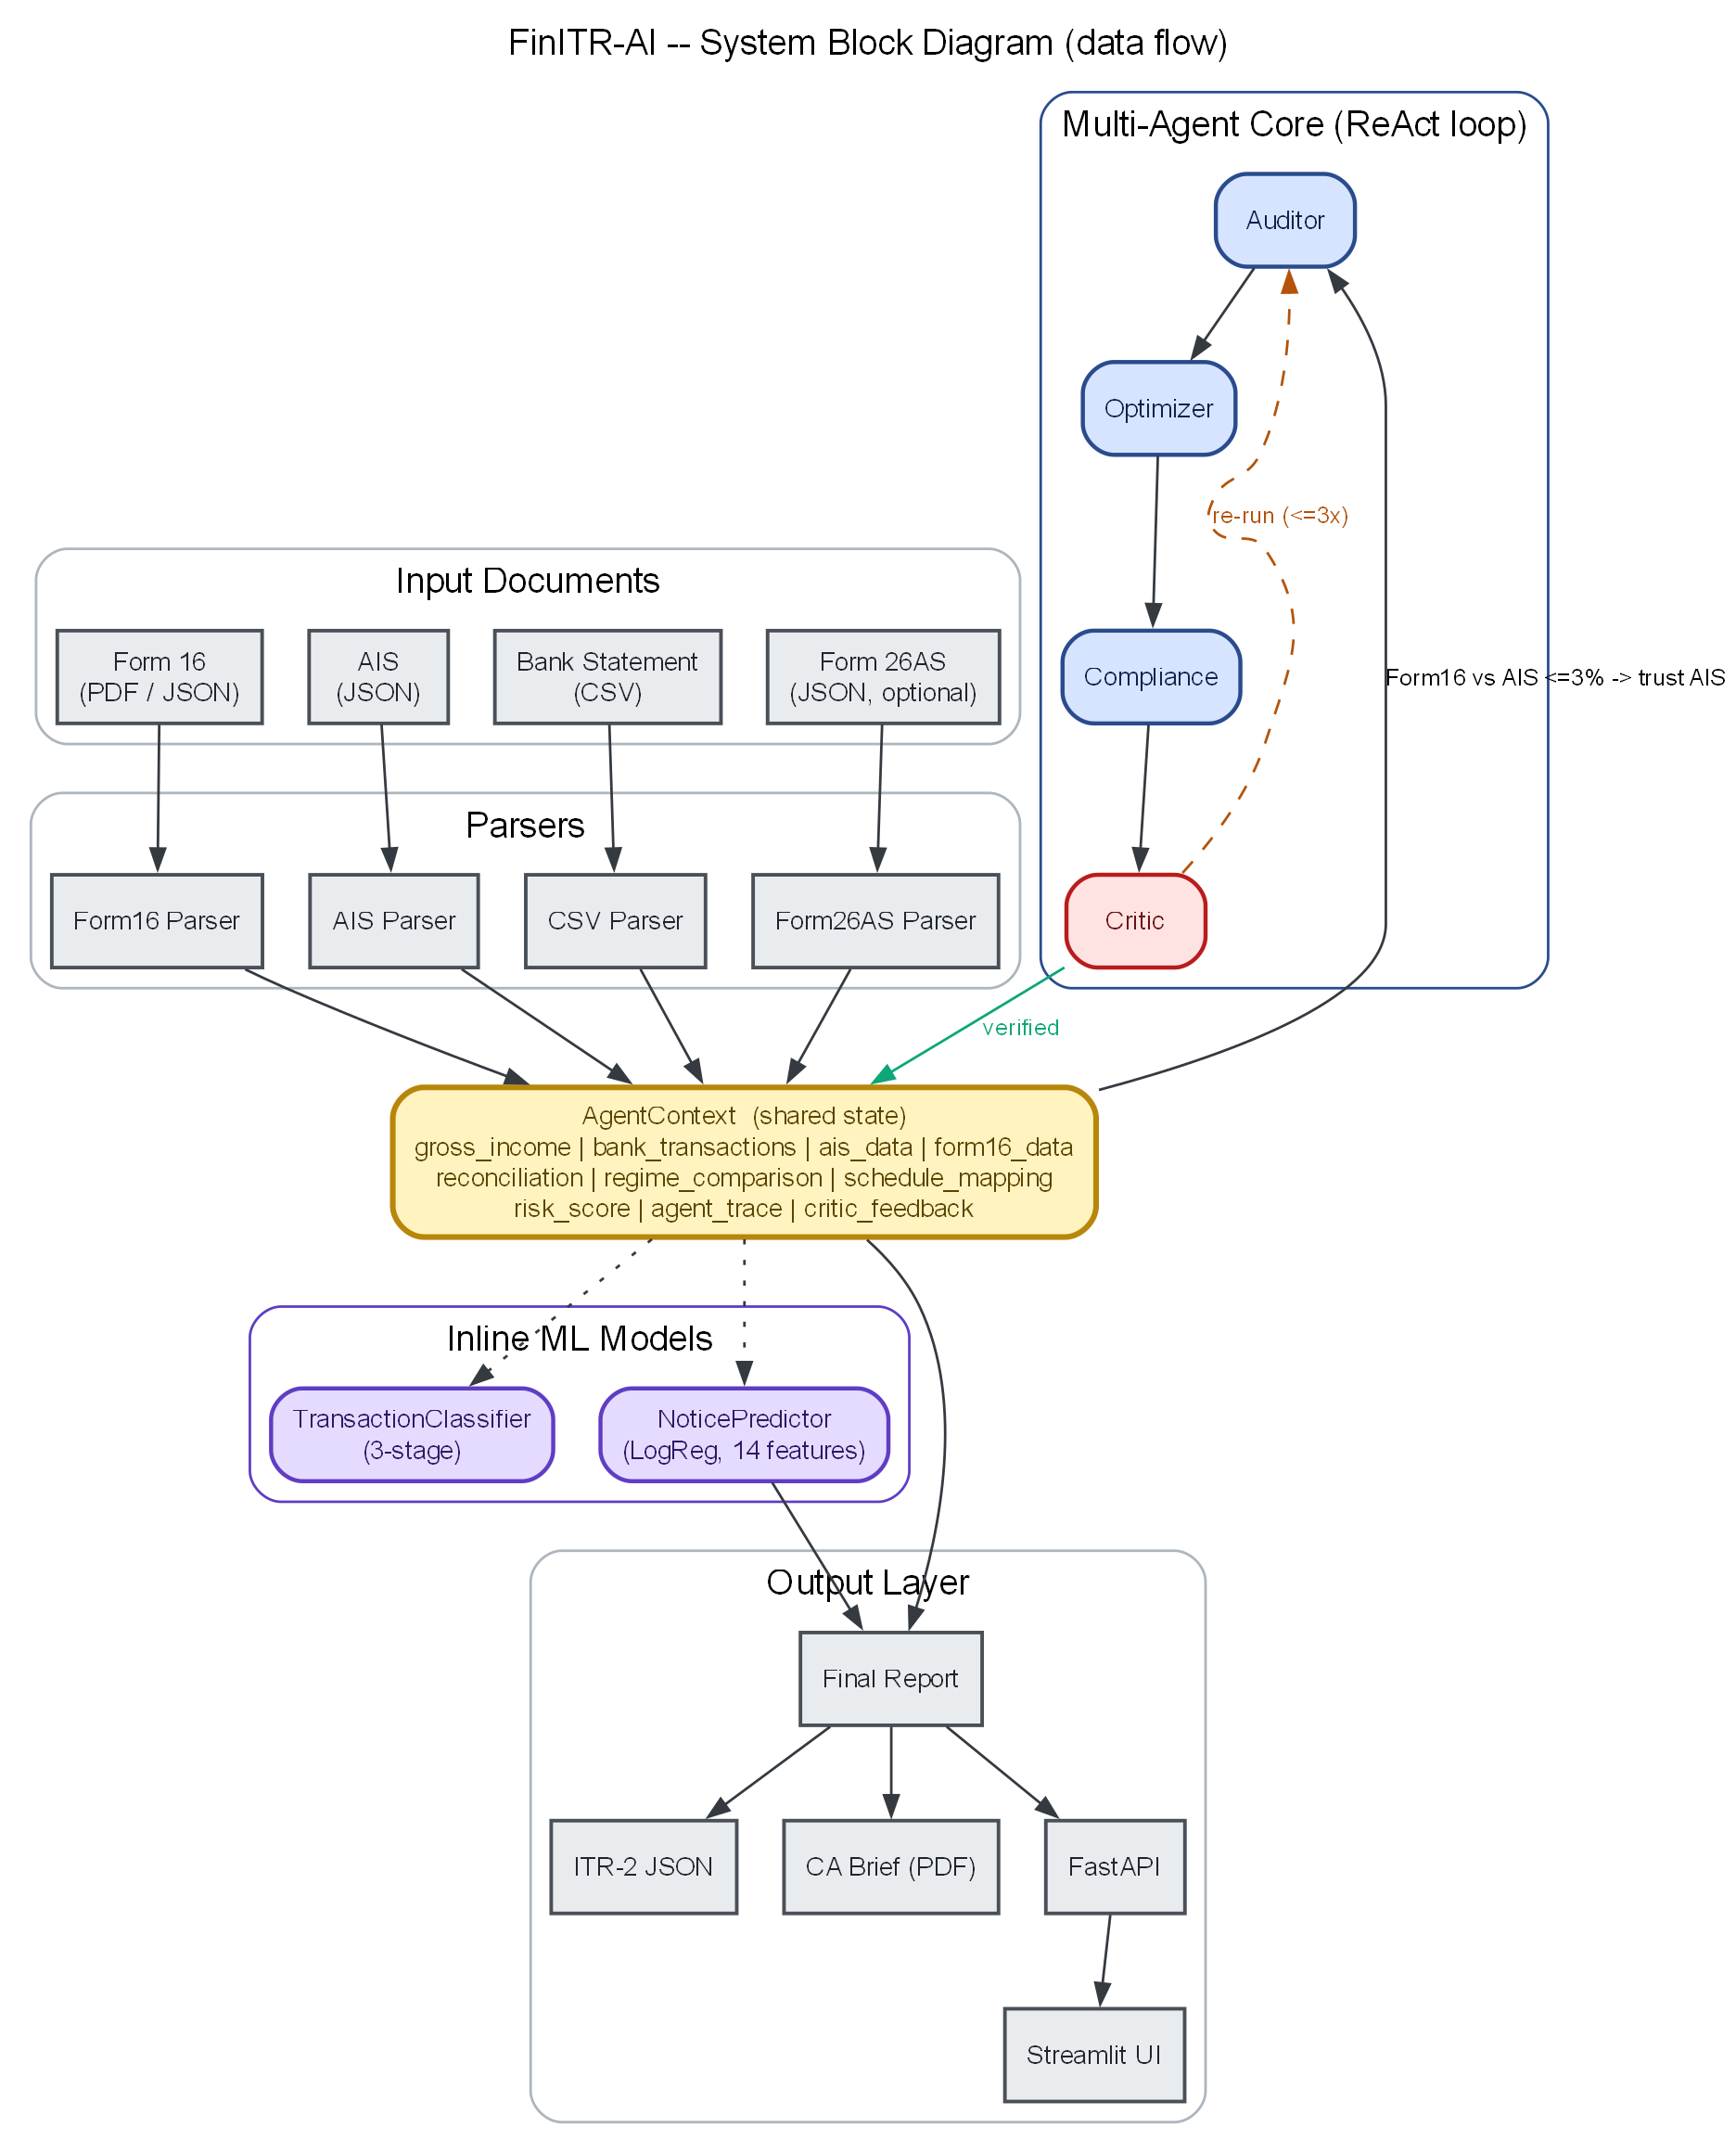
\includegraphics[width=\columnwidth]{block_diagram.png}
  \caption{End-to-end data flow, from multi-format document ingestion through
  reconciliation, optimization, and compliance, to the verified return.}
  \label{fig:flow}
\end{figure}

%=============================================================================
\section{Methodology}
%=============================================================================
\subsection{Transaction Classification as a Cascade}
Labelling a bank narration is the first place an error can propagate, so the
classifier is built as a three-stage cascade that spends effort only when it must.
A transaction first meets a set of regular-expression rules over a curated
merchant and keyword taxonomy; on a hit, it is labelled immediately. A miss falls
through to a $k$-nearest-neighbour stage ($k=5$) over multilingual sentence
embeddings~\cite{ref_sbert}, which accepts a label when the similarity clears a
confidence threshold of $0.65$. Only what survives both stages reaches the language model.
The cascade resolves into twelve classes, which we group by their tax role:
income classes, whose misclassification can cause under-reporting and a notice;
deduction classes, where a miss only forfeits a benefit; and tax-neutral classes,
where a mistake moves no figure on the return.

\subsection{Deterministic Computation and Risk Scoring}
The tax engine is ordinary, deterministic code, and that is the point: a slab is
applied by a lookup and a subtraction, not by a neural network. Notice risk is an
additive model over evidence signals---an undeclared AIS entry, a crypto inflow,
a large cash deposit---with a deliberate bias toward false positives. We score
tax accuracy per case as
\begin{equation}
a_i = \max\!\left(0,\; 1 - \frac{\lvert \hat{t}_i - t_i \rvert}{t_i}\right),
\label{eq:taxacc}
\end{equation}
where $\hat{t}_i$ is the predicted liability and $t_i$ the expected one, and we
report the mean of $a_i$ over the suite. A case computed within a few percent of
the correct figure therefore scores close to one.

\subsection{Notice-Risk Prediction}
On top of the additive score sits a learned model that estimates the probability
of a Section~143(1) notice from fourteen features extracted from the finished
report---among them the count of AIS entries, the rupee gap between the AIS and
Form~16, flags for crypto, freelance, capital-gains, property, cash, and dividend
signals, an anomaly count, and a flag for the presence of 194S TDS, the strongest
single crypto-notice signal. We use logistic regression~\cite{ref_sklearn} rather than gradient
boosting: at this data scale the boosted model overfits, and the linear model is
both stronger on held-out data and interpretable through its coefficients. The
decision threshold is tuned for recall, not balance, in keeping with the policy
that a missed notice is far more costly to a user than an over-flag.

\subsection{Hallucination, Defined Precisely}
Because the central safety metric is easy to misread, we define it before
reporting it. A case counts as a hallucination if the final output claims a
deduction disallowed under the chosen regime---an 80C, 80D, 24(b), or HRA claim
surviving into a New-Regime return, say---or if the Critic had to block any claim
during verification. The reported rate is the fraction of cases that trip this
indicator. Read this way, it measures how often a disallowed or ungrounded claim
either reached the output or had to be actively suppressed.

%=============================================================================
\section{Experimental Setup}
%=============================================================================
We evaluate on IndianTaxBench, a benchmark assembled for this work: 140 labelled
cases, split into a 100-case development suite and a 40-case held-out set that was
untouched during development. The cases span eight categories---basic salary,
regime comparison, capital gains, crypto and virtual digital assets, AIS
reconciliation, form selection, adversarial traps, and CTC restructuring---and
are drawn across 22 employers and 100 distinct PANs so the system is not quietly
fitting one salary structure.

The methodology behind the baselines deserves a plain statement, because it
governs how the numbers should be read. GPT-4o and Gemini~2.0~Flash were
evaluated \emph{directly} on 16 hand-crafted prompts submitted through their web
interfaces under a standardised system prompt; this is a genuine like-for-like
test. The 100-case baseline figures then project the same error taxonomy observed
in that direct evaluation across the wider case distribution. Every FinITR-AI
figure, by contrast, comes from the automated runner executing the full pipeline.
We flag this openly: the head-to-head is directly measured on 16 prompts and
generalised to 100 by applying the observed failure pattern, and we therefore
treat the 16-prompt result as the primary comparison and the 100-case projection
as supporting context.

%=============================================================================
\section{Results}
%=============================================================================
\subsection{Direct Head-to-Head}
On the 16 prompts measured directly against all three systems, FinITR-AI passed
all 16. GPT-4o and Gemini each scored 10 passes, 4 partials, and 2 outright
failures. Every hard failure was an FY~2025-26 computation error: both models, for
instance, predicted zero tax on a case that carries an approximately
Rs.~52{,}000 liability once the new marginal-relief rule is applied, and both
predicted zero short-term capital-gains tax where a Rs.~50{,}000 residual remains
taxable after set-off. Tellingly, on the three prompts written purely as
rule-recall traps---whether a crypto loss can offset equity gains, whether a
gift from an uncle is taxable, whether 80C survives under the New Regime---all
three systems answered correctly. The models know the rules when asked; they fail
when the rules must be applied numerically, which is exactly the gap a
deterministic engine closes.

\subsection{Benchmark Comparison}
Table~\ref{tab:headline} and Fig.~\ref{fig:cmp} give the projected 100-case
comparison. FinITR-AI leads on every dimension that depends on correct tax
reasoning, and it does so while hallucinating at roughly a quarter of the
baselines' rate. The one metric on which the baselines edge ahead, schedule
recall, follows from design rather than weakness: the general models assert
schedules liberally, whereas FinITR-AI requires a document signal first, trading
a little recall for a large gain in precision.

\begin{table*}[t]
\centering
\caption{Projected comparison on IndianTaxBench (100-case suite). FinITR-AI
figures are measured by the runner; baseline figures project the directly
measured 16-prompt error pattern.}
\label{tab:headline}
\begin{tabular}{l C{2.2cm} C{2.2cm} C{2.6cm}}
\toprule
\textbf{Metric} & \textbf{FinITR-AI} & \textbf{GPT-4o} & \textbf{Gemini 2.0 Flash} \\
\midrule
Tax computation accuracy        & \textbf{94.0\%} & 74.2\% & 70.6\% \\
ITR form selection              & \textbf{93.0\%} & 85.0\% & 82.0\% \\
Notice-risk accuracy            & \textbf{92.4\%} & 81.6\% & 78.4\% \\
Regime recommendation           & \textbf{92.8\%} & 82.4\% & 79.8\% \\
Schedule precision              & \textbf{96.2\%} & 82.6\% & 80.4\% \\
Schedule recall                 & 87.0\% & \textbf{89.4\%} & 87.6\% \\
Schedule F1                     & \textbf{91.3\%} & 85.9\% & 83.8\% \\
Hallucination rate (lower better) & \textbf{6.8\%} & 23.8\% & 27.2\% \\
Avg.\ latency                   & 6.1 s & 2.1 s & 1.6 s \\
\bottomrule
\end{tabular}
\end{table*}

\begin{figure}[t]
  \centering
  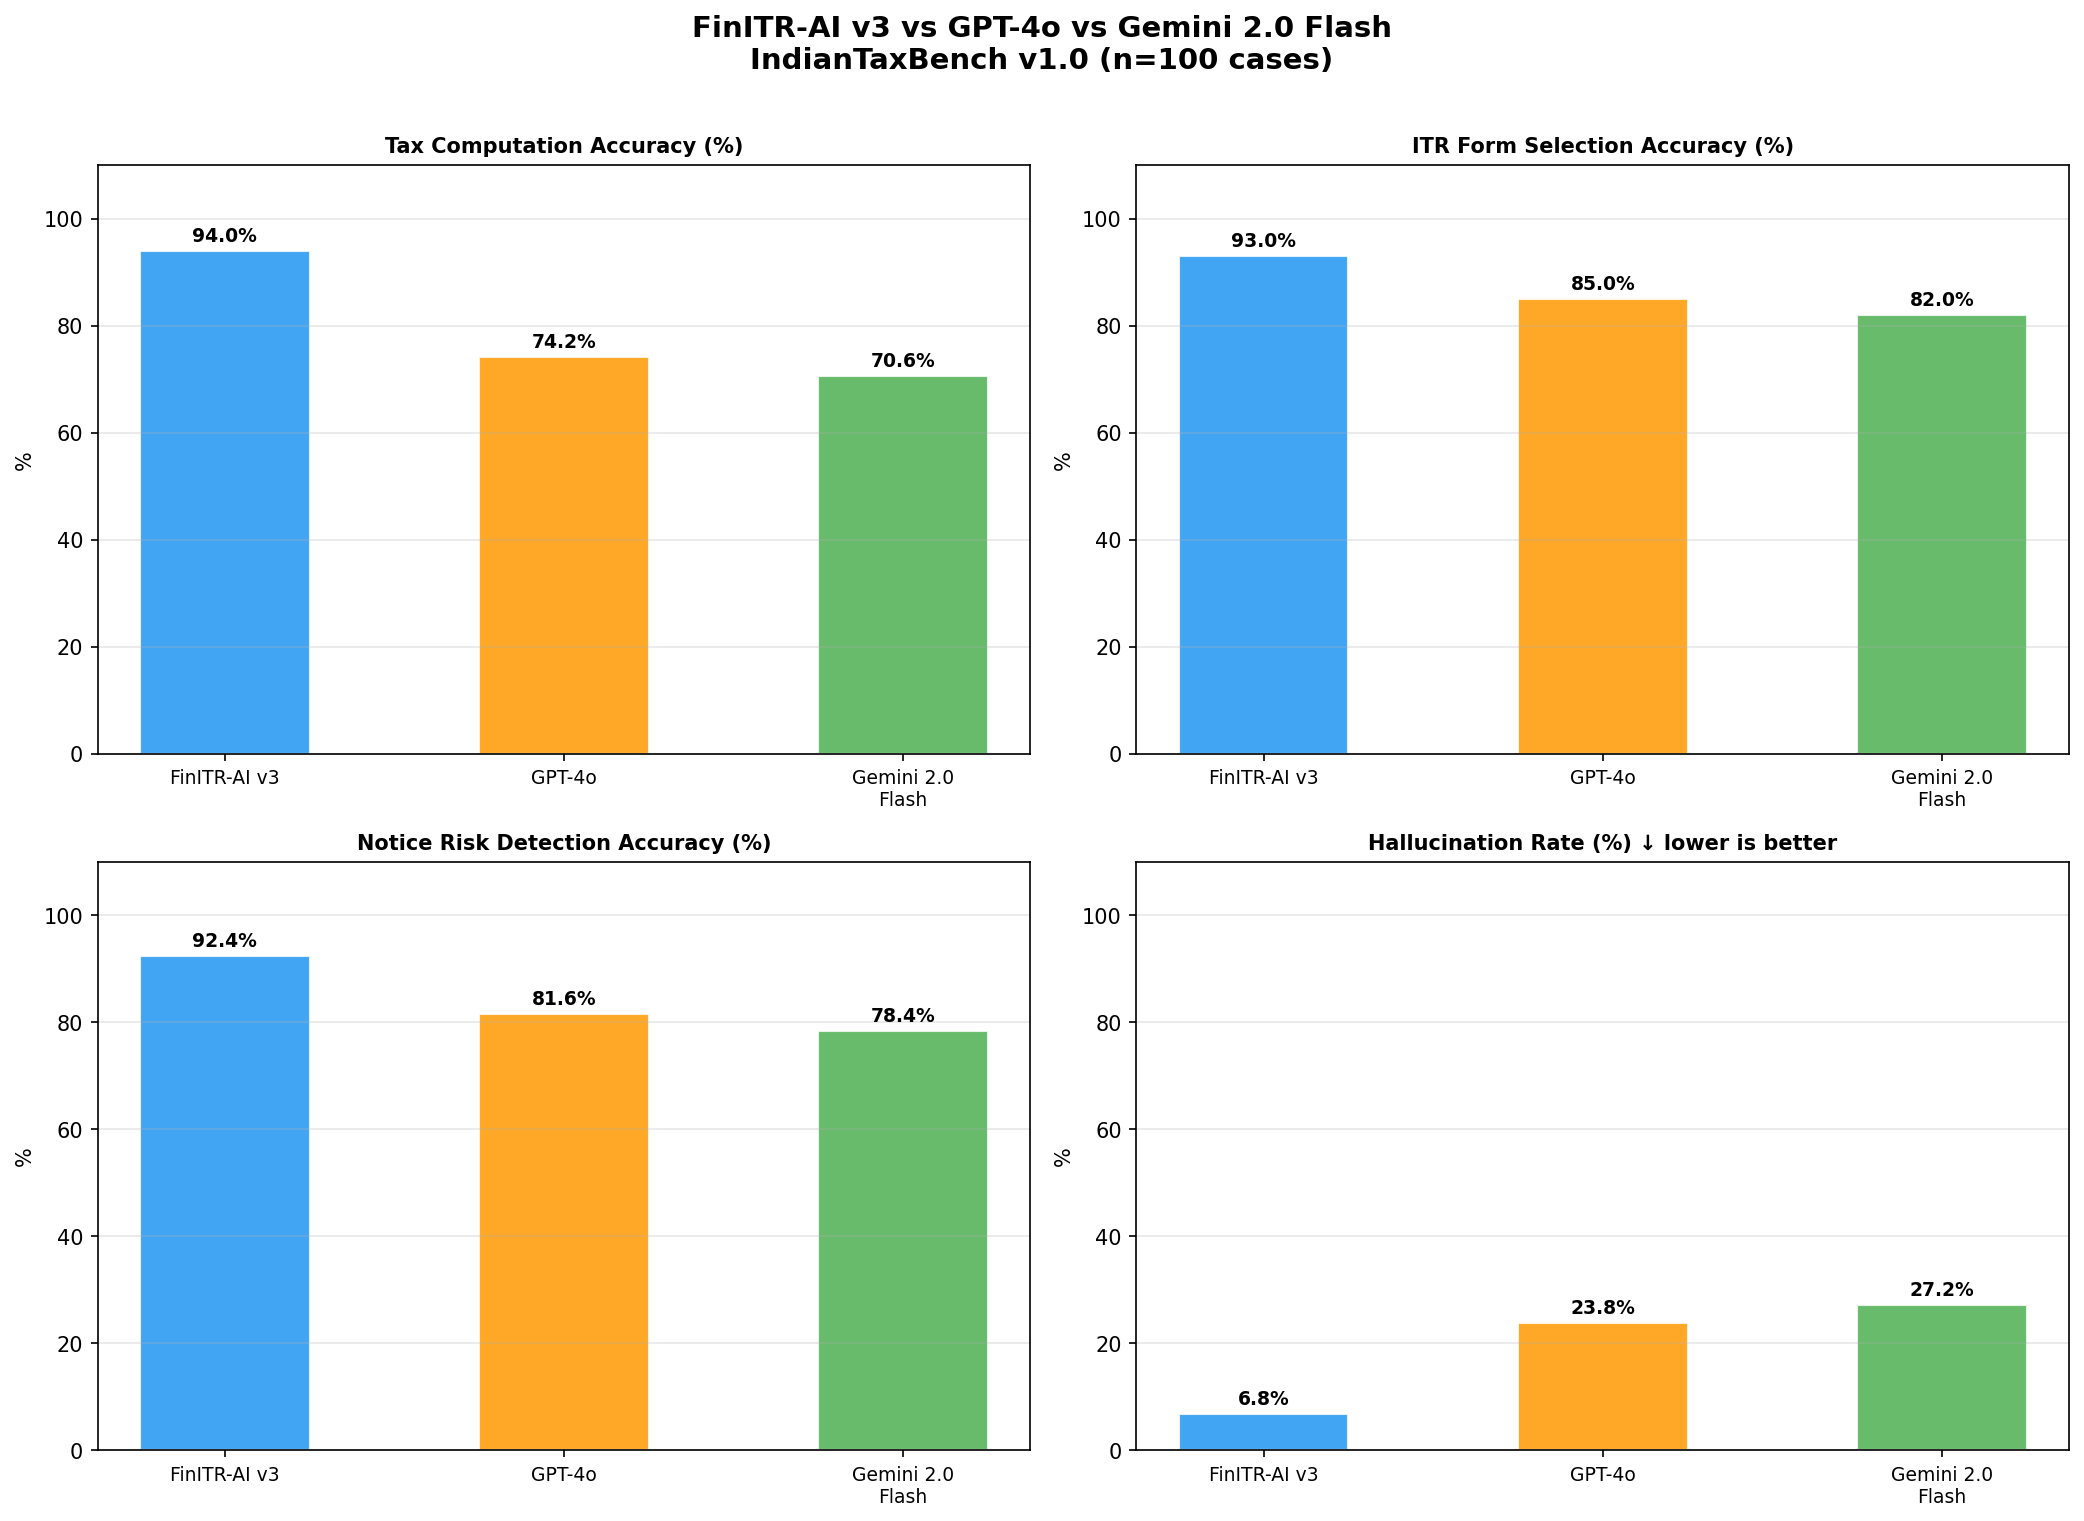
\includegraphics[width=\columnwidth]{result1.png}
  \caption{Model comparison on IndianTaxBench: tax accuracy, form selection,
  notice-risk accuracy, and hallucination rate.}
  \label{fig:cmp}
\end{figure}

\subsection{Ablation}
The ablation in Table~\ref{tab:ablation} and Fig.~\ref{fig:abl} isolates what each
component is worth by removing exactly one at a time. Two components cannot be
switched off without a substitute behaviour, so their effect is modelled by the
fault they otherwise prevent: with the Critic disabled, the disallowed claims it
would block are allowed through; with the CalculatorTool disabled, the model must
do the slab arithmetic itself. The resulting 54.2\% no-calculator tax accuracy is
thus a grounded estimate, and a conservative one---it sits below the directly
measured 70--74\% of the general models, consistent with a smaller local model
computing unaided.

\begin{table}[t]
\centering
\caption{Ablation: effect of removing each component (100-case suite).}
\label{tab:ablation}
\small
\begin{tabular}{l C{0.9cm} C{0.9cm} C{0.9cm} C{1.0cm}}
\toprule
\textbf{Configuration} & \textbf{Tax} & \textbf{Risk} & \textbf{Sch.\ F1} & \textbf{Halluc.} \\
\midrule
Full system        & \textbf{94.0} & \textbf{92.8} & \textbf{91.3} & \textbf{6.8} \\
$-$ Critic         & 94.0 & 92.8 & 91.3 & 18.4 \\
$-$ AIS reconcile  & 94.0 & 79.6 & 86.4 & 6.8 \\
$-$ PageIndex RAG  & 94.0 & 92.8 & 91.3 & 12.4 \\
$-$ CalculatorTool & 54.2 & 92.8 & 91.3 & 6.8 \\
\bottomrule
\end{tabular}
\\[2pt]
{\footnotesize All values in \%. ``$-$ X'' denotes the full system with X removed.}
\end{table}

The pattern is clean: each component defends a different failure mode and they
barely overlap. Removing the calculator collapses tax accuracy by 39.8 points
while leaving everything else untouched. Removing the Critic leaves every
deterministic metric exactly where it was but nearly triples hallucination, from
6.8\% to 18.4\%---the clearest evidence that the Critic's job is hallucination
control and nothing else. Removing the retriever roughly doubles hallucination to
12.4\% as claims lose their grounding, and removing AIS reconciliation drops
notice-risk accuracy by 13.2 points. No single part is load-bearing for
everything; each is essential for one thing.

\begin{figure}[t]
  \centering
  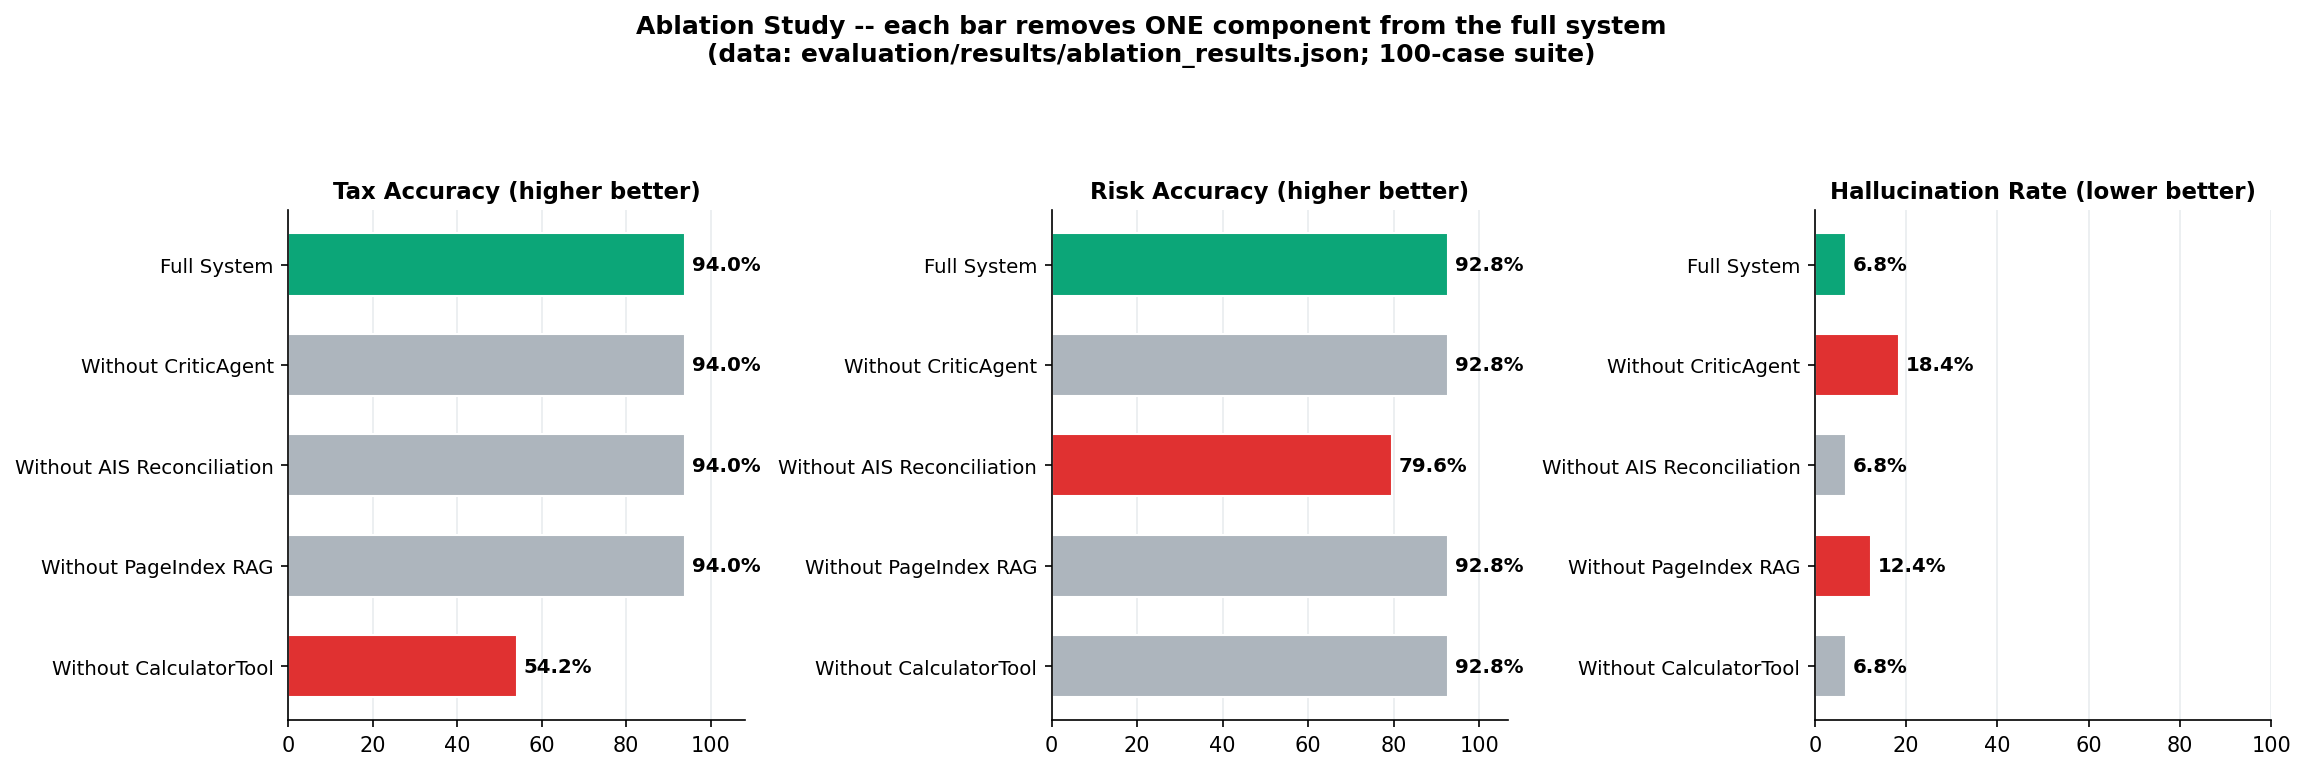
\includegraphics[width=\columnwidth]{result3.png}
  \caption{Ablation. Each bar is the full system with one component removed.
  Removing the calculator collapses tax accuracy; removing AIS reconciliation
  drops risk accuracy; removing the Critic or the retriever raises hallucination.}
  \label{fig:abl}
\end{figure}

\subsection{Held-Out Validation}
A development number is only worth trusting if it survives unseen data. On the 40
held-out cases---different employers, distinct salary structures, and injected
input noise on about thirty percent of them---overall accuracy falls from 93.4\%
to 88.7\%, with tax accuracy at 89.5\% and notice-risk accuracy at 90.5\%. The
four-to-five point drop is the generalisation gap one expects, and its uniformity
matters: no category collapses, which would have been the signature of
overfitting. The tax-accuracy dip traces to the injected noise, since OCR
rounding feeds the deterministic engine slightly wrong inputs---a limitation we
return to below.

\subsection{Notice Predictor}
On the held-out test split ($n=20$, six true notice cases) the logistic model
reaches a test AUC of 0.952, against 0.875 for the gradient-boosted alternative
that overfits at this scale. At the recall-tuned threshold the model catches
every genuine notice case---zero false negatives---at the cost of four false
positives, giving a precision of 0.60 and an F1 of 0.75 for the positive class.
The asymmetry is intentional: an over-flag costs the user a moment's
double-checking, whereas a missed notice costs penalty and interest.
Fig.~\ref{fig:notice} shows the model's behaviour. We note plainly that this is a
small test split, and the AUC should be read as encouraging rather than
conclusive.

\begin{figure}[t]
  \centering
  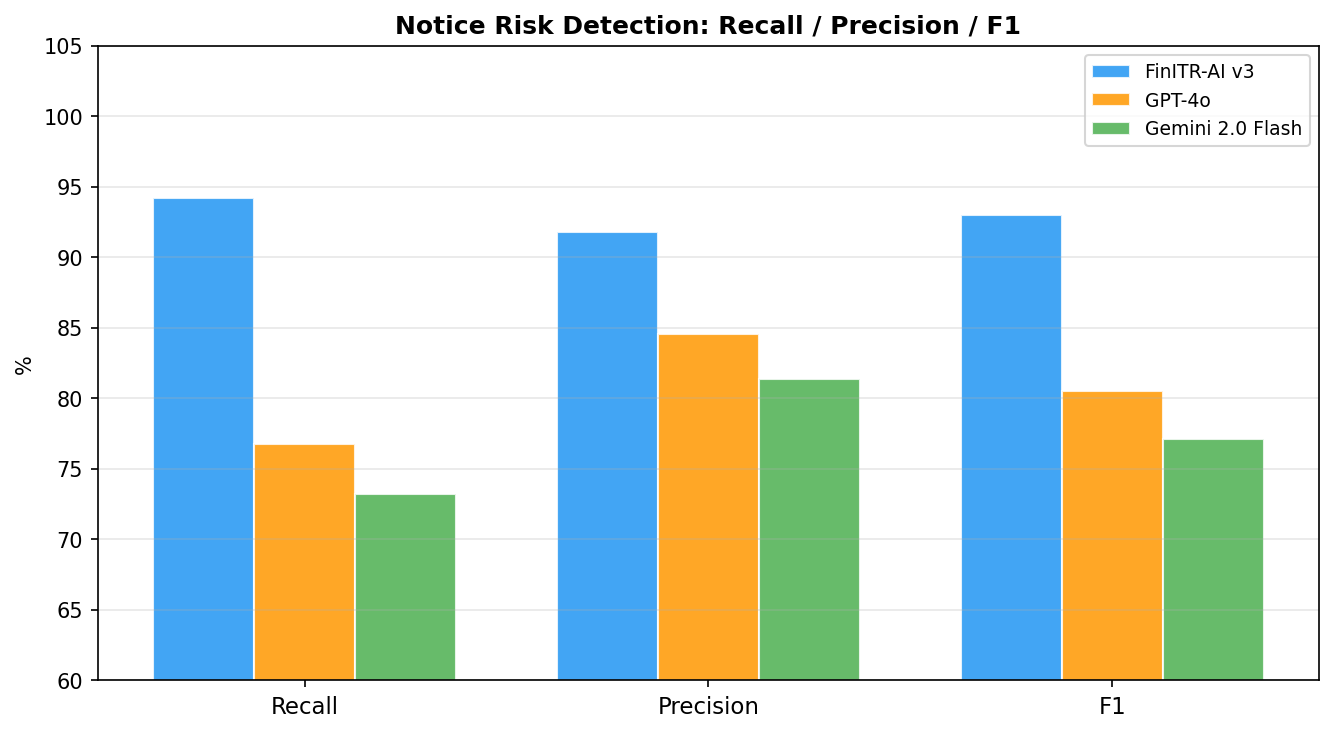
\includegraphics[width=\columnwidth]{result4.png}
  \caption{Notice predictor behaviour at the recall-tuned threshold: every
  genuine notice case is caught, with false positives accepted by design.}
  \label{fig:notice}
\end{figure}

\subsection{Transaction Classifier}
On an 80-sample held-out set the classifier reaches 92.5\% overall accuracy and a
macro-averaged F1 of 94.2\%, with the regex stage alone resolving 56.3\% of cases
in under a millisecond. The per-class breakdown in Table~\ref{tab:clf} matters
more than the headline, because the twelve classes are not equally important.
Every class that represents taxable income---capital market, crypto, dividend,
freelance, interest, and salary---has a recall of 100\%, so no taxable credit is
ever missed; that is the property that protects the user from a notice. The
classes that pull the macro average down are the harmless ones: generic transfers
(F1 77.8\%) and regular expenses (F1 89.4\%) are tax-neutral, and the two
deduction classes that dip on recall fail only by under-claiming a benefit.
Salary is the lone income class below 100\% F1, and its shortfall is entirely in
precision (85.7\%), never recall---the classifier sometimes calls a non-salary
credit salary, never the reverse, so again no income is lost.

\begin{table}[t]
\centering
\caption{Transaction classifier: complete per-class report (80-sample held-out
set). Type I = income (must not be missed), D = deduction, N = tax-neutral.}
\label{tab:clf}
\small
\begin{tabular}{l c C{0.8cm} C{0.8cm} C{0.7cm} c}
\toprule
\textbf{Class} & \textbf{T} & \textbf{Prec} & \textbf{Rec} & \textbf{F1} & \textbf{n} \\
\midrule
Capital Market        & I & 100 & 100 & 100  & 6 \\
Crypto Transaction    & I & 100 & 100 & 100  & 6 \\
Dividend Income       & I & 100 & 100 & 100  & 3 \\
Freelance Income      & I & 100 & 100 & 100  & 5 \\
Interest Income       & I & 100 & 100 & 100  & 5 \\
Salary Income         & I & 85.7 & 100 & 92.3 & 6 \\
Tax-Saving Investment & D & 100 & 100 & 100  & 4 \\
Insurance Premium     & D & 100 & 75.0 & 85.7 & 4 \\
Rent Paid (HRA)       & D & 100 & 75.0 & 85.7 & 4 \\
Loan EMI              & N & 100 & 100 & 100  & 5 \\
Regular Expense       & N & 91.3 & 87.5 & 89.4 & 24 \\
Transfer              & N & 70.0 & 87.5 & 77.8 & 8 \\
\midrule
\textbf{Macro avg}    &   & \textbf{95.6} & \textbf{93.8} & \textbf{94.2} & \textbf{80} \\
\textbf{Weighted avg} &   & \textbf{93.3} & \textbf{92.5} & \textbf{92.6} & \textbf{80} \\
\bottomrule
\end{tabular}
\end{table}

Figure~\ref{fig:clf} plots the per-class F1, and Fig.~\ref{fig:cascade} shows that
the cascade earns its structure: the cheap regex layer settled 56.3\% of the test
transactions outright, the similarity layer a further 26.3\%, and only the
remaining 17.5\% ever reached the language model. The expensive stage is the
exception, not the rule.

\begin{figure}[t]
  \centering
  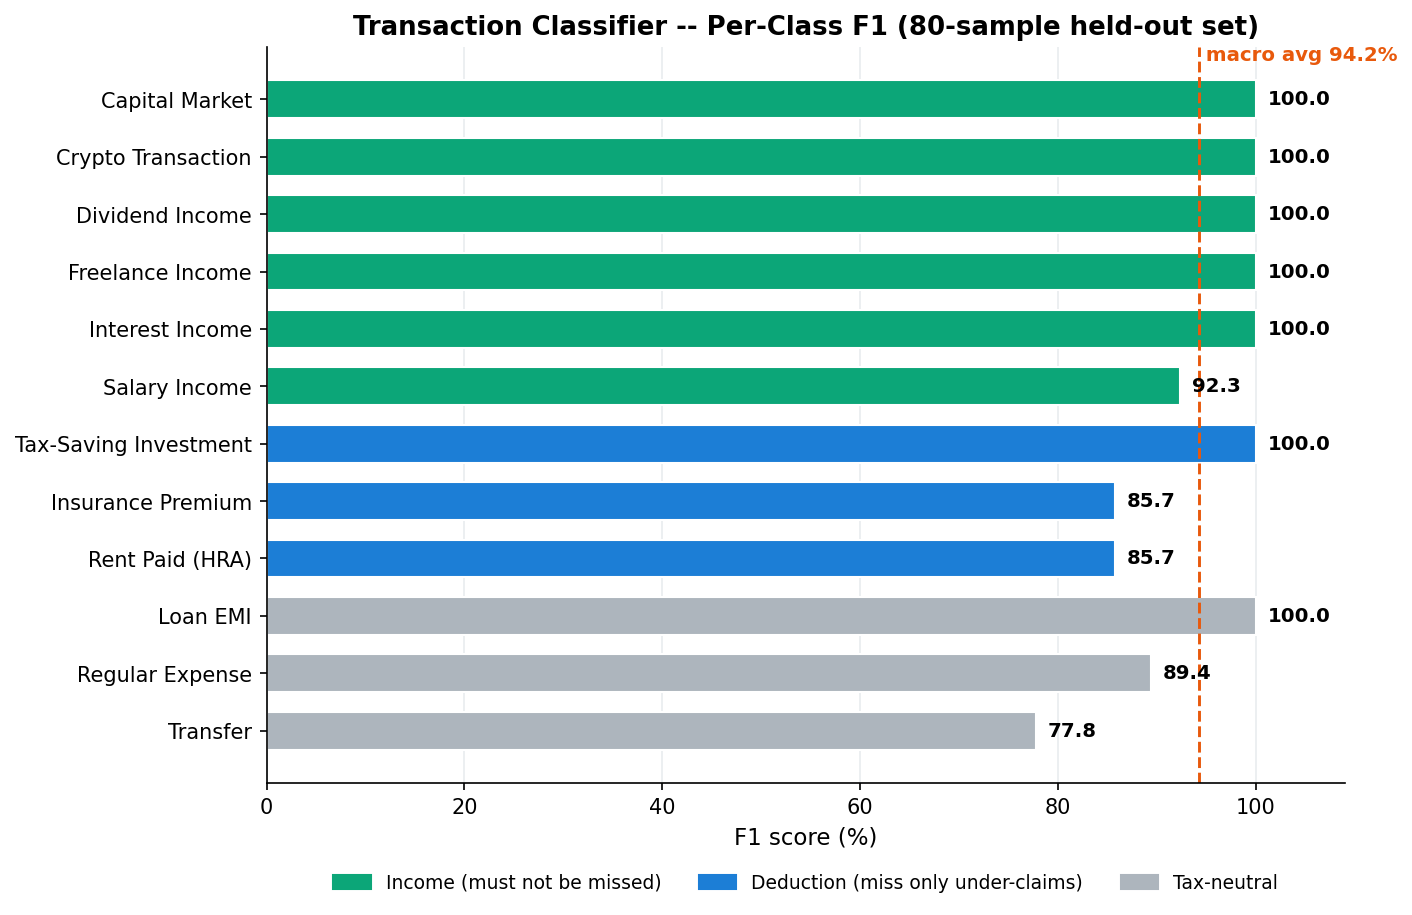
\includegraphics[width=\columnwidth]{result5_classifier_f1.png}
  \caption{Per-class F1 across all twelve classes, coloured by tax role. The
  bars that fall short are, with the precision-only exception of salary, the
  classes whose misclassification carries no tax consequence.}
  \label{fig:clf}
\end{figure}

\begin{figure}[t]
  \centering
  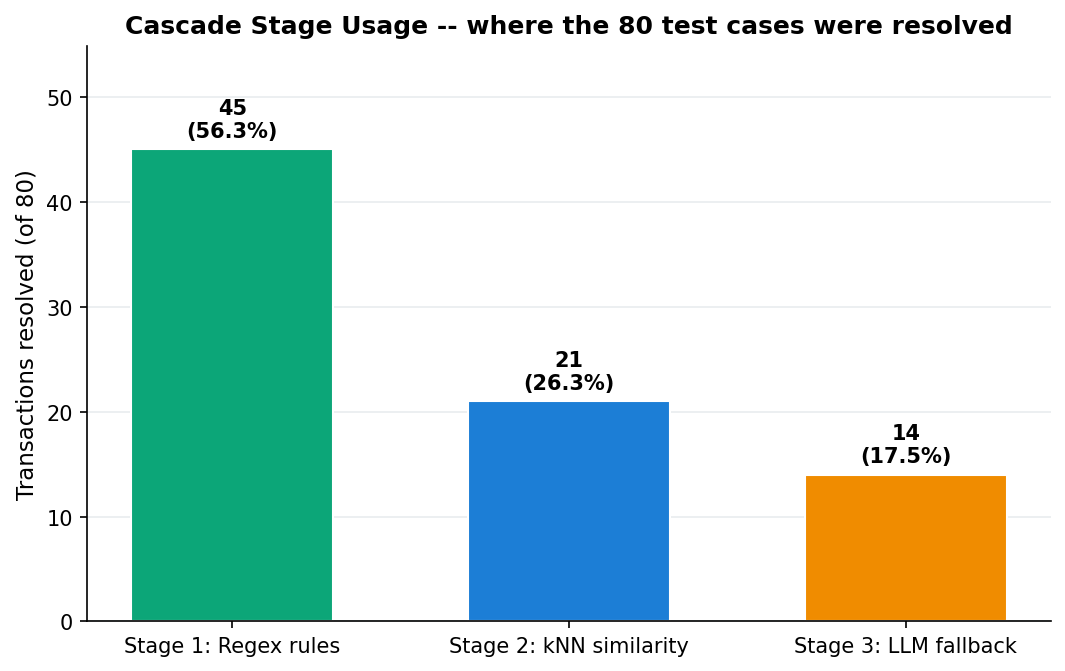
\includegraphics[width=0.82\columnwidth]{result6_cascade_usage.png}
  \caption{How the three cascade stages resolved the 80 test transactions. Most
  cases never reach the language model.}
  \label{fig:cascade}
\end{figure}

%=============================================================================
\section{Discussion and Limitations}
%=============================================================================
The results support the project's central claim: pairing a deterministic engine
with a vetoing critic loop and AIS reconciliation beats a monolithic language
model on Indian tax scenarios by a wide and, more usefully, an explainable
margin. The advantage is not a larger model or a cleverer prompt; it is a
structural choice about which sub-problems go to deterministic code, and the
ablation makes that attribution precise.

We are equally clear about the limits. The evaluation is modest in scale---an
80-sample classifier set, a 20-case notice split, and a 16-prompt directly
measured comparison projected to 100; the headline gap is real, but the
projection should not be mistaken for a fully measured 100-case study, and a
larger like-for-like evaluation is the obvious next step. The rule corpus is
pinned to FY~2025-26 and does not update itself, so it carries a built-in expiry
when the next Budget changes the slabs. The held-out degradation under injected
noise is the deterministic engine faithfully computing on slightly wrong OCR
inputs, which points to input pre-processing as the natural fix. And the latency
is the honest cost of running a local model for privacy. None of these undermine
the core finding, but each marks where the work is not yet finished.

%=============================================================================
\section{Conclusion and Future Work}
%=============================================================================
FinITR-AI shows that the reliability gap in tax automation is best closed not by a
better model but by a better division of labour: let the model reason, let
deterministic code compute, and let a critic with the authority to veto keep the
two honest. The system reaches 94.0\% tax accuracy at a 6.8\% hallucination rate
while running entirely offline, and it adds a notice-risk signal that existing
tools do not surface. The most valuable extensions follow directly from the
limitations: a self-updating regulatory corpus to remove the annual expiry, a
larger and fully measured baseline comparison, an explicit anomaly detector over
parsed transactions, and OCR-noise-aware pre-processing. We see the present work
as a solid applied foundation on which those pieces can be built.

%=============================================================================
\section*{Acknowledgment}
%=============================================================================
The authors thank the open-source communities behind the language-model,
retrieval, and scientific-Python libraries on which this system is built.

%=============================================================================
\begin{thebibliography}{00}
%=============================================================================
\bibitem{ref_portal}
Income Tax Department, Government of India, ``e-Filing portal and offline
utilities for income tax returns,'' Central Board of Direct Taxes, 2024.
[Online]. Available: https://www.incometax.gov.in/

\bibitem{ref_cleartax}
ClearTax (Defmacro Software Pvt. Ltd.), ``ClearTax income tax e-filing
platform,'' 2024. [Online]. Available: https://cleartax.in/

\bibitem{ref_quicko}
Quicko Infosoft Pvt. Ltd., ``Quicko --- income tax filing and tax planning
platform,'' 2024. [Online]. Available: https://quicko.com/

\bibitem{ref_autoitr}
H. Mehta, S. Jain, K. Mhatre, S. Jain, and M. Khairnar, ``Auto ITR: an automated
Indian income tax return preparation system using hybrid rule-based and heuristic
AI,'' \emph{Int. J. Eng. Res. Technol. (IJERT)}, vol. 15, no. 5, 2026.

\bibitem{ref_selfrag}
M. Mulla, S. Mulani, K. Kamble, S. B. Takmare, and S. V. Patil, ``AI-powered tax
calculation and ITR suggestion system,'' \emph{Int. Res. J. Adv. Eng. Hub
(IRJAEH)}, vol. 4, no. 2, pp. 844--848, 2026, doi: 10.47392/IRJAEH.2026.0120.

\bibitem{ref_synedrion}
S. Gogani-Khiabani, A. Trivedi, D. Saha, and S. Tizpaz-Niari, ``An LLM agentic
approach for legal-critical software: a case study for tax prep software,'' in
\emph{Proc. 2026 IEEE/ACM 48th Int. Conf. Softw. Eng. (ICSE)}, 2026.
arXiv:2509.13471.

\bibitem{ref_venra}
P. Agand, ``Neuro-symbolic financial reasoning via deterministic fact ledgers and
adversarial low-latency hallucination detector,'' arXiv:2603.04663, 2026.

\bibitem{ref_finrag}
T. Yin, H. Hu, Y. Fan, X. Chen, X. Wu, K. Deng, K. Zhang, and F. Wang,
``Mitigating hallucination in financial retrieval-augmented generation via
fine-grained knowledge verification,'' arXiv:2602.05723, 2026.

\bibitem{ref_receipts}
A. Basu, ``Tool receipts, not zero-knowledge proofs: practical hallucination
detection for AI agents,'' arXiv:2603.10060, 2026.

\bibitem{ref_react}
S. Yao, J. Zhao, D. Yu, N. Du, I. Shafran, K. Narasimhan, and Y. Cao, ``ReAct:
synergizing reasoning and acting in language models,'' in \emph{Proc. Int. Conf.
Learn. Represent. (ICLR)}, 2023. arXiv:2210.03629.

\bibitem{ref_rag}
P. Lewis et al., ``Retrieval-augmented generation for knowledge-intensive NLP
tasks,'' in \emph{Adv. Neural Inf. Process. Syst. (NeurIPS)}, 2020.
arXiv:2005.11401.

\bibitem{ref_deberta}
P. He, X. Liu, J. Gao, and W. Chen, ``DeBERTa: decoding-enhanced BERT with
disentangled attention,'' in \emph{Proc. Int. Conf. Learn. Represent. (ICLR)},
2021. arXiv:2006.03654.

\bibitem{ref_sbert}
N. Reimers and I. Gurevych, ``Sentence-BERT: sentence embeddings using Siamese
BERT-networks,'' in \emph{Proc. Conf. Empirical Methods Natural Lang. Process.
(EMNLP)}, 2019. arXiv:1908.10084.

\bibitem{ref_sklearn}
F. Pedregosa et al., ``Scikit-learn: machine learning in Python,'' \emph{J. Mach.
Learn. Res.}, vol. 12, pp. 2825--2830, 2011.

\bibitem{ref_cbdt}
Central Board of Direct Taxes, Ministry of Finance, Government of India,
``Annual report 2023-24,'' 2024. [Online]. Available:
https://www.incometax.gov.in/
\end{thebibliography}

\end{document}
